\documentclass[11pt]{report}

\usepackage[top=2.0cm]{geometry}
\usepackage[sort&compress]{natbib}
\usepackage{url}
\usepackage{graphics}
\usepackage{graphicx}
\usepackage{textcomp}
\usepackage{gensymb}
\usepackage[format=hang,font=scriptsize]{caption}
\usepackage{subcaption}
\usepackage{placeins}
\usepackage{needspace}
\usepackage{wrapfig}
\usepackage{csquotes}
\usepackage{sidecap}
\usepackage{subfloat}
\usepackage{framed}
\usepackage{lipsum}
\usepackage{subfiles}
\usepackage[english]{isodate}
\usepackage{cleveref}

\bibliographystyle{plain}

\title{  Derivative Analysis of Data Sets \\
  \large BSc (Honours) Project Report
}
\author{S\"onke W\"ohler  \\
  University of Aberdeen }
\date{2019}    

\begin{document}
  
  \begin{titlepage}
    \begin{center}
    \vspace*{2.0cm}

    \huge
    \textbf{Derivative Analysis of Data Sets} \\
    \LARGE
    BSc (Hons.) Project Report    \\
    \vspace{1.5cm}
    \Large
    \textbf{S\"onke W\"oher}\\
    \large
    University of Aberdeen     \\
    \vspace{1.5cm}
    2019
    
    
    \begin{figure}[h!]
      \centering
      
\includegraphics{otherImages/abdnshield}
      \caption*{}
    \end{figure}
    
    \vfill
    \end{center}
    I declare that this document and the accompanying code has been composed by myself, and describes my own work, unless otherwise acknowledged in the text. It has not been accepted in any previous application for a degree. All verbatim extracts have been distinguished by quotation marks, and all sources of information have been specifically acknowledged.
    \\\\
    Signed: 
    \hfill 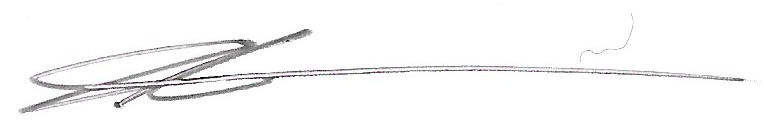
\includegraphics[height=0.78cm]{otherImages/sonkiSignature}\hspace{2.5cm}
    \\
    S\"onke W\"ohler \hfil \today
  \end{titlepage} 
  
  \begingroup
    \fontsize{8pt}{10pt}\selectfont
  
      \lipsum[1]
  
  \endgroup
  \hrulefill
  
  \section*{Acknowledgements}
  
  % Can also include
    % Terminology
    % Abbreviations
    % Notations
  
  \clearpage
  \tableofcontents
  
  \chapter{Introduction}
    % motivation
    % intentions
  
  \chapter{Background and Inception}
    % building on introduction
    % place within bigger picture of Analysis Project
    % clarify its role within the project 
      % Data Format
      % Trace by Trace Analysis (TTA)
      % Synthetic Data?
  
  \chapter{Concepts}
    % Data Structure
    % Trace by Trace Anaysis
      % Points of Interest
      % Polynomal
      % Exponential
    % Limitations
      % Trigonometric
        % Use FFT
      % Nested Functions
      % Noise vs Precision
        % Typical Trade Off
      % Processing
  
  \chapter{Implementation}
    % Technologies
      % Issue with J11 and J in general
    % ? Software Development
      % ? Architectural Patterns
      % Requirements ???
    % Synthetic Data
      % For testing and demonstration
      % also useful for future maybe ? 
    % Presentation    
    % ? Verification ?
      % Synthetic Data
      % Processing ?
      % Reliability
        % works largely as expected
      % ? Real Well Data 
    % gracefully address problems (points for honesty)
    
  \chapter{Conclusion}
  
  \chapter{User Manual}
  
  \chapter{Maintenance Manual}
  
  \chapter{Code PDF}
  
  
  \clearpage
  \nocite{*} % remove before final submission
  \bibliography{refs-main}
  


\end{document}  
